\documentclass{article}

\usepackage[spanish]{babel} % Establece el idioma español
\usepackage{csquotes} % Carga el paquete csquotes
\usepackage{graphicx} % Required for inserting images
\usepackage{listings}
\usepackage{xcolor}
\usepackage{hyperref}
\usepackage[left=1.00cm, right=1.00cm, top=2.00cm, bottom=2.00cm]{geometry}
\usepackage{tikz}
\usetikzlibrary{shapes,arrows}
\usetikzlibrary{positioning}
\setlength{\parindent}{0.5in}
\usepackage{setspace}
\doublespacing

\lstset{
  basicstyle=\ttfamily,
  columns=fullflexible
}

% Define colores para el código
\definecolor{codegreen}{rgb}{0,0.6,0}
\definecolor{codegray}{rgb}{0.5,0.5,0.5}
\definecolor{codepurple}{rgb}{0.58,0,0.82}
\definecolor{backcolour}{rgb}{0.95,0.95,0.92}

% Configuración de lstlisting
\lstdefinestyle{mystyle}{
    backgroundcolor=\color{backcolour},   
    commentstyle=\color{codegreen},
    keywordstyle=\color{magenta},
    numberstyle=\tiny\color{codegray},
    stringstyle=\color{codepurple},
    basicstyle=\ttfamily\footnotesize,
    breakatwhitespace=false,         
    breaklines=true,                 
    captionpos=b,                    
    keepspaces=true,                 
    numbers=left,                    
    numbersep=5pt,                  
    showspaces=false,                
    showstringspaces=false,
    showtabs=false,                  
    tabsize=2
}

% Configuración del paquete hyperref
\hypersetup{
    colorlinks=true,
    linkcolor=black,
    filecolor=magenta,      
    urlcolor=gray,
}

\lstset{style=mystyle}

\renewcommand{\baselinestretch}{1.5}

\newtheorem{propo}{Proposición}[section]
\newtheorem{lema}[propo]{Lema}
\newtheorem{teo}[propo]{Teorema}
\newtheorem{coro}[propo]{Corolario}

\newtheorem{defi}[propo]{Definición}
\newtheorem{obs}[propo]{Observación}
\newtheorem{ejemplo}[propo]{Ejemplo}
\newtheorem{ejercicio}[propo]{Ejercico}

\newcommand{\sol}{\textbf{Solución}}

\title{Apache Kafka}
\author{Kevin Cárdenas}
\date{Febrero 2023}

\begin{document}
\begin{titlepage}
\begin{center}
{\Huge \textbf{Apache Kafka}}
\\[18cm]

\large\emph{Autor:}\\
Kevin Cárdenas.
\\[1cm]
{\large Enero de 2023}

\end{center}
\end{titlepage}
\newpage
\tableofcontents
\newpage
\section{Introducción}
En la actualidad, existe una gran cantidad de aplicaciones y sistemas que requieren la capacidad de procesar y almacenar grandes cantidades de datos en tiempo real. Para abordar esta necesidad, surgió Kafka, una plataforma de procesamiento de flujos de datos en tiempo real.\\

Kafka es una herramienta altamente escalable, distribuida y tolerante a fallas, que permite a los usuarios producir y consumir eventos a través de una serie de tópicos. Un tópico es un canal virtual que permite la transmisión de mensajes de un productor a un consumidor. Cada mensaje es almacenado en un servidor llamado Broker, y puede ser consumido en cualquier momento por un consumidor.\\

En resumen, Kafka es una plataforma clave para el procesamiento en tiempo real de grandes cantidades de datos, y los conceptos de productor, consumidor, tópico, offset, broker y cluster son fundamentales para comprender su funcionamiento y aprovechar al máximo su potencial.\\

\subsection{Conceptos Básicos}
\begin{defi}\textbf{Productor}\\
Un productor de Kafka es una aplicación o sistema que escribe datos
en un tópico de Kafka.
\end{defi}

\begin{defi}\textbf{Consumidor}\\
Un consumidor de Kafka es una aplicación o sistema que lee los datos de uno o varios topicos de Kafka.
\end{defi}

\begin{defi}\textbf{Un Broker de kafka}\\
Un broker de Kafka es un servidor que forma parte del cluster y se encarga de almacenar y transmitir los datos de los tópicos.
\end{defi}

\begin{defi}\textbf{Un cluster de Kafka}\\
Un cluster de Kafka es un grupo de brokers que trabajan juntos para gestionar la distribución de datos en los tópicos de Kafka. Es posible tener varios brokers en un cluster para aumentar la capacidad y la disponibilidad del sistema.
\end{defi}

\begin{defi}\textbf{tópico}\\
Un tópico de Kafka es una categoría lógica en la que los datos son publicados y suscritos.
\end{defi}
\begin{defi}\textbf{El offset de Kafka}\\
El offset de Kafka es una marca numérica que indica el lugar de un registro en un tópico. Es utilizado por los consumidores para rastrear su progreso en la lectura de datos.

\end{defi}

\begin{defi}
    \textbf{Partition}\\
    Cada topic se divide en particiones, estas son la unidad de paralelismo dentro de kafka, se debe especificar el número de particiones que requerimos para el topic cuando lo creamos, también podemos especificar el tiempo que queremos que se almacene los datos (7 días por defecto), cuando hay más de una partición los datos se dividen entre las particiones y en diferentes brokers.
\end{defi}

\begin{defi}\textbf{TCP }\\
TCP es un acrónimo de -Protocolo de Control de Transmisión-. Es un protocolo de comunicación de nivel de transporte que se utiliza para garantizar la fiabilidad de las comunicaciones de red. Proporciona una conexión confiable y ordenada para la transmisión de datos entre dispositivos.
\end{defi}

\begin{defi}\textbf{HTTP}\\
HTTP es el acrónimo de -HyperText Transfer Protocol-. Es un protocolo de comunicación para la transmisión de información en la World Wide Web. Se utiliza para recibir y enviar información entre el navegador web y un servidor web.
\end{defi}

\begin{defi}\textbf{RPC}\\
RPC es un acrónimo de -Remote Procedure Call Protocol-. Es un tipo de protocolo de comunicación que permite a un programa en un sistema enviar una solicitud a un programa en otro sistema (en la misma red o en una red diferente) y esperar una respuesta. Este protocolo se utiliza para llevar a cabo procedimientos remotos en un sistema distribuido.
\end{defi}

\subsection{Contextualización}
Un productor es un componente que envía mensajes a un tópico en Kafka, mientras que un consumidor es un componente que se suscribe a uno o varios tópicos para recibir mensajes. Los mensajes en un tópico son almacenados en una secuencia y son asignados un offset único, lo que permite a los consumidores llevar un registro de los mensajes que han sido procesados y los que aún no han sido procesados.\\

Kafka funciona como un cluster de múltiples brokers, lo que permite una alta disponibilidad y escalabilidad. Además, los brokers mantienen una copia de los mensajes en varios servidores, lo que garantiza la durabilidad de los datos.\\

Kafka es un sistema de mensajería en tiempo real diseñado para ser altamente escalable, confiable y rápido. Está diseñado para manejar grandes cantidades de datos en tiempo real, lo que lo hace ideal para una variedad de usos, incluyendo la gestión de eventos, el seguimiento de métricas y la integración de sistemas.\\

Un concepto clave en Kafka es el de \textbf{Productores}. Los productores son aplicaciones que envían mensajes a los tópicos en un cluster de Kafka. Cada mensaje contiene una clave y un valor que pueden ser procesados por una aplicación de consumidor.\\

Los \textbf{Consumidores} son aplicaciones que consumen los mensajes de los tópicos de un cluster de Kafka. Un consumidor pertenece a un grupo de consumidores y se asigna a una partición específica dentro de un tópico. Cada partición contiene una secuencia de mensajes que pueden ser leídos por un solo consumidor en el grupo.\\

Los \textbf{Tópicos} son las divisiones lógicas dentro de un cluster de Kafka que almacenan los mensajes. Cada mensaje enviado a un tópico se divide entre las particiones asociadas con ese tópico.\\

El \textbf{Offset} es la posición de un mensaje dentro de una partición de un tópico. Este valor se utiliza para identificar de manera única un mensaje dentro de una partición y para permitir a los consumidores marcar su progreso a través de la partición.\\

Los \textbf{Brokers} son los servidores que forman parte de un cluster de Kafka y almacenan y transmiten los mensajes. Un cluster de Kafka está compuesto por varios brokers que trabajan juntos para garantizar la alta disponibilidad y la escalabilidad del sistema.\\

En resumen, Kafka es un sistema de mensajería en tiempo real con una arquitectura escalable y confiable, que se compone de productores, consumidores, tópicos, offsets, brokers y clusters. Cada uno de estos conceptos es importante para entender cómo Kafka funciona y cómo se puede utilizar para resolver diferentes problemas de negocios.
\newpage
\section{El origen del Streaming}
La Figura 2-1 muestra un sistema de procesamiento de flujos utilizado para ingerir datos de varios cientos de miles de dispositivos móviles. Cada dispositivo envía pequeños mensajes JSON para
denotar aplicaciones en cada móvil que se están abriendo, cerrando o se bloquean. Esto se puede utilizar para buscar inestabilidad, es decir, cuando la proporción de caídas con respecto al uso es comparativamente alta.\\
\begin{center}
    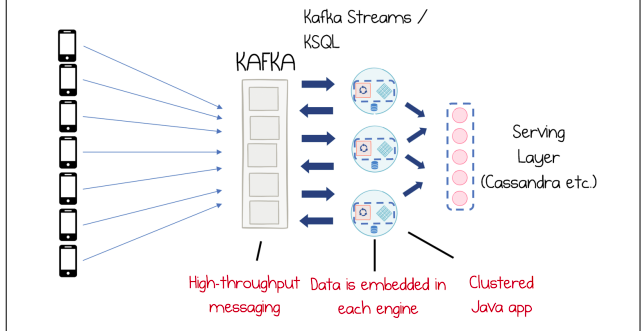
\includegraphics[scale=0.8]{figure2.1.png}
    Figura 2-1\\
    -Extracto del libro 'Designing Event-Driven Systems' por Ben Stopford, publicado por O'Reilly Media, Inc. Copyright © 2018 O'Reilly Media. Todos los derechos reservados.-
\end{center}
Los dispositivos móviles envían sus datos a Kafka, que los almacena en búfer hasta que pueden ser extraídos por las distintas aplicaciones que necesitan utilizarlos. Para este
tipo de carga de trabajo, el clúster sería relativamente grande.
Ingiere datos a la velocidad de la red, pero la sobrecarga de la replicación normalmente divide
por tres (por lo que un clúster de tres nodos 10 GbE ingiere alrededor de 1 GB/s en la práctica).\\

A la derecha de Kafka en la Figura 2-1 se sitúa la capa de procesamiento de flujos. Se trata de una aplicación clustered, donde las consultas se definen por adelantado a través del DSL de Java o
dinámicamente a través de KSQL, el lenguaje de procesamiento de flujos tipo SQL de Kafka. A diferencia de una
base de datos tradicional, estas consultas se calculan de forma continua, por lo que
cada vez que llega una entrada a la capa de procesamiento de flujos, se vuelve a calcular la consulta y se emite un resultado si el valor de la entrada es correcto.\\

Una vez que un nuevo mensaje ha pasado por todos los cálculos de streaming, el resultado
aterriza en una capa de servicio desde la que se puede consultar. Como se muestra en la
Figura 2-1, pero empujando a HDFS (Hadoop Distributed File System), empujando a
otro almacén de datos, o consultar directamente desde Kafka Streams utilizando su función de
interactiva también son enfoques comunes.\\

Para entender mejor el streaming, es útil observar una consulta típica. La Figura 2-2
muestra una que calcula el número total de caídas de aplicaciones al día. Cada vez que llega un
nuevo mensaje que indique que una aplicación se ha bloqueado, el recuento total de bloqueos de esa aplicación se incrementará. Tenga en cuenta que este cálculo
requiere estado: el recuento para el día hasta ahora (es decir, dentro de la duración de la ventana)
para que, si el procesador de flujo se bloquea o reinicia, el recuento continúe donde estaba antes. Kafka Streams y KSQL gestionan este estado internamente, y ese estado se respalda en Kafka a través de un tema de registro de cambios.
\begin{center}
    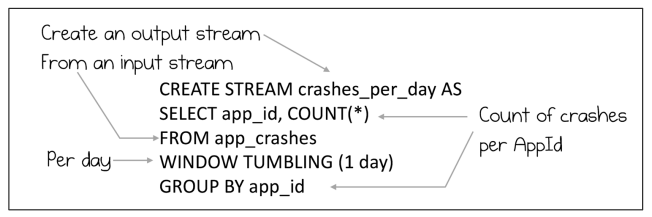
\includegraphics[scale=0.8]{figure2.2.png}
    Figura 2-2\\
    -Extracto del libro 'Designing Event-Driven Systems' por Ben Stopford, publicado por O'Reilly Media, Inc. Copyright © 2018 O'Reilly Media. Todos los derechos reservados.-
\end{center}
En la figura 2-3, resolvimos el problema anterior en tres pasos encadenados en dos etapas. Las consultas (a) y (b) calculan continuamente las aplicaciones abiertas por día y las aplicaciones que han fallado por día, respectivamente. Los dos flujos de salida resultantes se combinan en la etapa final (c), que calcula la estabilidad de la aplicación al calcular la relación entre los fallos y el uso y compararla con un límite fijo.\\
\begin{center}
    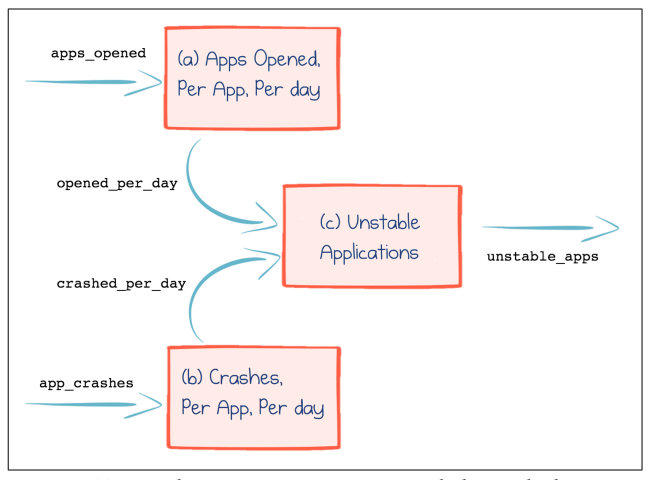
\includegraphics[scale=0.8]{figure2.3.png}
    Figura 2-3\\
    -Extracto del libro 'Designing Event-Driven Systems' por Ben Stopford, publicado por O'Reilly Media, Inc. Copyright © 2018 O'Reilly Media. Todos los derechos reservados.-
\end{center}
Además de lo que se ha mencionado, hay algunas otras cosas que deben tenerse en cuenta sobre este enfoque de transmisión en tiempo real:
\begin{itemize}
    \item La capa de transmisión es tolerante a fallos: se ejecuta como un clúster en todos los nodos disponibles. Si un nodo sale, otro continuará donde lo dejó. Del mismo modo, se puede escalar el clúster agregando nuevos nodos de procesamiento. El trabajo y cualquier estado requerido se redirigirán automáticamente para hacer uso de estos nuevos recursos.
    \item Cada nodo de procesador de flujo puede tener su propio estado: esto es necesario para el almacenamiento en búfer, así como para mantener tablas completas, por ejemplo, para realizar enriquecimientos. Esta idea de almacenamiento local es importante, ya que permite al procesador de flujo realizar consultas rápidas de un mensaje a la vez sin cruzar la red, una característica necesaria para las cargas de trabajo de alta velocidad vistas en casos de uso a escala de internet. Pero esta capacidad de internalizar el estado en almacenes locales resulta útil para un número de casos de uso relacionados con los negocios también.
\end{itemize}
Este capítulo se enfoca en brindar una introducción a los sistemas de procesamiento de stream y cómo funcionan. Se describen las características típicas de una aplicación de streaming, que consiste en la ingestión de datos de dispositivos móviles en Kafka, el procesamiento de los datos en una capa de streaming y luego la emisión de resultados a una capa de almacenamiento donde se pueden realizar consultas. Se explica el funcionamiento de una consulta típica, que calcula el número total de fallos de la aplicación por día. Cada vez que llega un nuevo mensaje, que indica un fallo de la aplicación, se incrementará el conteo de fallos totales. Se describen algunas características adicionales de este enfoque de streaming, como la tolerancia a fallos, la capacidad de almacenar estado local en cada nodo de procesador de stream y la capacidad de escribir y almacenar estado local.\\

En resumen, este capítulo proporciona una introducción básica a los sistemas de procesamiento de stream y sus características clave, lo que ayuda a comprender mejor cómo funcionan y cómo se utilizan en aplicaciones de streaming.\\
\newpage
\section{¿Es Kafka Lo Que Piensas Que Es?}
Hay un antiguo parábola sobre un elefante y un grupo de hombres ciegos. Ninguno de los hombres había visto un elefante antes. Un hombre ciego se acerca a la pierna y declara: -Es como un árbol-. Otro hombre se acerca a la cola y declara: -Es como una cuerda-. Un tercero se acerca a la trompa y declara: -Es como una serpiente-. Por lo tanto, cada hombre ciego percibe al elefante desde su punto de vista específico y llega a una conclusión ligeramente diferente sobre lo que es un elefante. Por supuesto, el elefante es como todas estas cosas, ¡pero en realidad es solo un elefante!
De manera similar, cuando las personas aprenden sobre Kafka a menudo lo ven desde un punto de vista determinado.\\ 

Estas perspectivas suelen ser precisas, pero solo destacan alguna subsección de toda la plataforma. En este capítulo examinamos algunos puntos de vista comunes.
\subsection{¿Kafka es como REST, pero Asíncrono?}
Kafka ofrece un protocolo asíncrono para conectar programas entre sí, pero es sin duda un poco diferente de, por ejemplo, TCP, HTTP o un protocolo RPC. La diferencia es la presencia de un corredor. Un corredor es una pieza separada de infraestructura que transmite mensajes a cualquier programa que esté interesado en ellos, así como los almacena por tanto tiempo como sea necesario. Entonces, es perfecto para el flujo de transmisión.\\

Otros casos de uso se encuentran más lejos de su terreno de origen. Un buen ejemplo es la respuesta a una solicitud. Digamos que tiene un servicio para consultar información de clientes. Llamas a un método getCustomer (), pasándole un CustomerId, y obtienes un documento que describe a un cliente en la respuesta. Puede construir este tipo de interacción de solicitud-respuesta con Kafka usando dos temas: uno que transporta la solicitud y uno que transporta la respuesta. La gente construye sistemas así, pero en tales casos el corredor no contribuye tanto. No hay ningún requisito de transmisión. Tampoco hay ningún requisito de almacenamiento. Entonces, surge la pregunta: ¿sería mejor utilizar un protocolo sin estado como HTTP?\\

Entonces, Kafka es un mecanismo para que los programas intercambien información, pero su terreno de origen es la comunicación basada en eventos, donde los eventos son hechos comerciales que tienen valor para más de un servicio y vale la pena mantenerlos.
\subsection{¿Kafka es como un sistema de mensajería?}
Kafka es como un sistema de mensajería, y con su interfaz Connect, que extrae y envía datos a una amplia gama de interfaces y almacenes de datos, y las APIs de transmisión en tiempo real que pueden manipular los datos en tránsito, parece similar a un ESB (bus de servicios empresariales). La diferencia es que los ESBs se enfocan en la integración de sistemas legados y comercializados, utilizando una capa de mensajería efímera y de bajo rendimiento, lo que fomenta los protocolos de solicitud-respuesta.\\

Por otro lado, Kafka es una plataforma de transmisión en tiempo real y, como tal, se centra en eventos de alta capacidad y procesamiento de flujos de datos. Un clúster de Kafka es en su corazón un sistema distribuido, proporcionando alta disponibilidad, almacenamiento y escalabilidad lineal. Esto es bastante diferente a los sistemas de mensajería tradicionales, que están limitados a una sola máquina o, si escalan hacia fuera, estas propiedades de escalabilidad no se extienden de extremo a extremo. Herramientas como Kafka Streams y KSQL permiten escribir programas simples que manipulan los eventos a medida que se mueven y evolucionan. Esto hace que las capacidades de procesamiento de una base de datos estén disponibles en la capa de aplicación a través de una API y fuera de las restricciones del intermediario compartido.\\

En algunos círculos, los ESBs son criticados debido a la forma en que la tecnología se ha construido durante los últimos 15 años, especialmente cuando los ESBs son controlados por equipos centrales que dictan esquemas, flujos de mensajes, validación e incluso transformación. En la práctica, los enfoques centralizados como este pueden restringir a una organización, dificultando que las aplicaciones y servicios individuales evolucionen a su propio ritmo.\\

ThoughtWorks hizo un llamado recientemente a los usuarios para evitar recrear los problemas vistos en los ESBs con Kafka, y al mismo tiempo, el empresa alentó a los usuarios a investigar la transmisión de eventos como fuente de verdad. Ambos representan consejos sensatos.\\

Hay una similitud entre Kafka y un sistema de mensajería como un autobús de servicio empresarial (ESB, por sus siglas en inglés). Sin embargo, hay diferencias importantes. Mientras que los ESBs se enfocan en la integración de sistemas heredados y comprados, utilizando una capa de mensajería efímera y con una capacidad de baja tasa de transferencia, Kafka es una plataforma de transmisión en tiempo real que se enfoca en eventos y procesamiento de transmisiones de alta tasa. Un cluster de Kafka es un sistema distribuido que proporciona alta disponibilidad, almacenamiento y escalabilidad lineal. Además, herramientas como Kafka Streams y KSQL permiten escribir programas simples para manipular eventos a medida que se desplazan y evolucionan, lo que hace que las capacidades de procesamiento de una base de datos estén disponibles en la capa de aplicación, a través de una API, fuera de las limitaciones del intermediario compartido. Aunque puede parecer que Kafka es similar a un ESB, en realidad es muy diferente y ofrece una tasa de transferencia, disponibilidad y almacenamiento mucho más altos. En resumen, Kafka permite a las aplicaciones y servicios tener control sobre sus propios datos y evolucionar a su propio ritmo, en lugar de ser controlados por un equipo central.

\subsection{¿Kafka es como una base de datos?}
Se dice que a veces Kafka se compara con una base de datos. De hecho, tiene características similares. Ofrece almacenamiento; no es infrecuente encontrar temas de producción con cientos de terabytes. Tiene una interfaz SQL que permite a los usuarios definir consultas y ejecutarlas sobre los datos contenidos en el registro. Estas se pueden enviar a vistas que los usuarios pueden consultar directamente. También admite transacciones. ¡Estos son todos aspectos que suenan bastante -base de datos-!
Sin embargo, aunque muchos de los elementos de una base de datos tradicional están presentes, Kafka es más bien una base de datos al revés (ver -Una base de datos al revés- en la página 89 en el capítulo 9), una herramienta para almacenar datos, procesarlos en tiempo real y crear vistas. Y aunque está perfectamente autorizado para colocar un conjunto de datos en Kafka, ejecutar una consulta KSQL sobre él y obtener una respuesta, al igual que lo haría en una base de datos tradicional, KSQL y Kafka Streams están optimizados para el cálculo continuo en lugar del procesamiento por lotes.\\

Por lo tanto, aunque la analogía no es completamente incorrecta, está un poco fuera de lugar. Kafka está diseñado para mover datos, operando en esos datos mientras lo hace. Se trata primero del procesamiento en tiempo real y en segundo lugar del almacenamiento a largo plazo.

\subsection{¿Qué es Kafka realmente? Una plataforma de streaming}
Kafka es una plataforma de transmisión. En su núcleo se encuentra un grupo de intermediarios de Kafka. Puede interactuar con el grupo a través de una amplia gama de API's de clientes en Go, Scala, Python, REST, y más. Hay dos API para el procesamiento de flujos: Kafka Streams y KSQL. Estos son motores de base de datos para los datos en tránsito, permitiendo a los usuarios filtrar flujos, unirlos, agregarlos, almacenar estados y ejecutar funciones arbitrarias sobre el flujo de datos en evolución. Estas API pueden ser con estado, lo que significa que pueden mantener tablas de datos como una base de datos regular. La tercera API es Connect. Este tiene un completo ecosistema de conectores que se comunican con diferentes tipos de bases de datos u otros endpoints, tanto para extraer datos como para enviar datos a Kafka. Finalmente, hay una suite de utilidades, como Replicator y Mirror Maker, que unen grupos dispares, y el Schema Registry, que valida y administra los esquemas, aplicados a los mensajes pasados a través de Kafka y una serie de otros herramientas en la plataforma Confluent. Una plataforma de streaming reúne estas herramientas con el propósito de convertir los datos en reposo en datos que fluyen a través de una organización.\\

A menudo se utiliza la analogía de un sistema nervioso central. La capacidad de la intermediación de escalar, almacenar datos y ejecutarse sin interrupción la convierte en una herramienta única para conectar muchas aplicaciones y servicios dispares a través de un departamento o organización. La interfaz Connect hace que sea fácil evolucionar lejos de los sistemas heredados, desbloqueando conjuntos de datos ocultos y convirtiéndolos en flujos de eventos. El procesamiento de flujo permite que las aplicaciones y servicios incorporen lógica directamente sobre estos flujos resultantes de eventos.
\begin{center}
    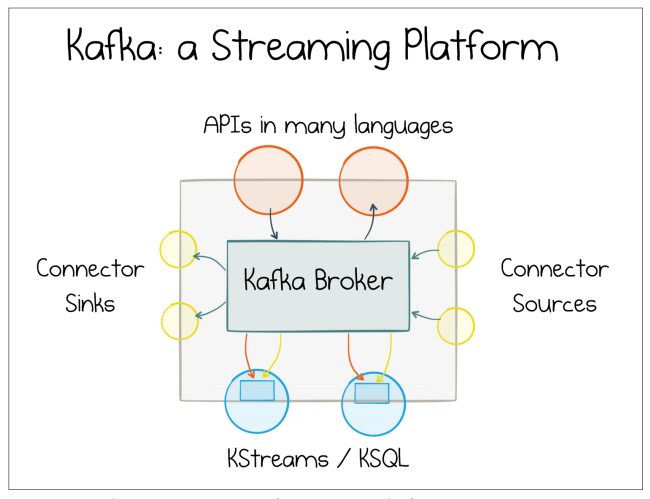
\includegraphics[scale=0.8]{figure3.1.png}
    Figura 3-1\\
    -Extracto del libro 'Designing Event-Driven Systems' por Ben Stopford, publicado por O'Reilly Media, Inc. Copyright © 2018 O'Reilly Media. Todos los derechos reservados.-
\end{center}

\newpage
\section{Más allá de la mensajería: una descripción general del Kafka Broker}
El sistema Kafka es básicamente una colección de archivos llenos de mensajes que se extienden en varias máquinas diferentes. La mayor parte del código de Kafka se ocupa de unir estos diversos registros individuales, encaminar mensajes de los productores a los consumidores de forma confiable, replicar para tener tolerancia a fallos y manejar los fallos de manera eficaz. Por lo tanto, es un sistema de mensajería, al menos en cierto sentido, pero es bastante diferente de los brokers de mensajería que lo precedieron. Al igual que cualquier tecnología, tiene sus ventajas y desventajas, y esto influye en el diseño de los sistemas que escribimos. Este capítulo examina el broker Kafka (es decir, el componente del servidor) desde el contexto de la construcción de sistemas comerciales. Exploraremos un poco sobre cómo funciona, así como también entraremos en los usos menos convencionales que soporta, como el almacenamiento de datos, el fallo dinámico y la protección de ancho de banda.\\

Originalmente construido para distribuir los conjuntos de datos creados por grandes redes sociales, Kafka fue predominantemente moldeado por la necesidad de funcionar a gran escala, en presencia de fallos. En consecuencia, su arquitectura hereda más de sistemas de almacenamiento como HDFS, HBase o Cassandra que de los sistemas de mensajería tradicionales que implementan JMS (Java Message Service) o AMQP (Advanced Message Queuing Protocol).\\

Al igual que muchos buenos resultados en la informática, esta escalabilidad se debe en gran parte a la simplicidad. La abstracción subyacente es un registro particionado, esencialmente un conjunto de archivos solo para agregar que se extienden en un número de máquinas, lo que fomenta patrones de acceso secuencial que fluyen naturalmente con la dirección del hardware subyacente.\\

El clúster de Kafka es un sistema distribuido que se extiende en varias máquinas para garantizar la tolerancia a fallos y escalabilidad lineal. Este sistema está diseñado para manejar una variedad de usos, desde la transmisión de alta velocidad, donde solo importan los últimos mensajes, hasta casos críticos de misión donde los mensajes y su orden relativo deben preservarse con las mismas garantías que se esperan de un sistema de gestión de bases de datos o de almacenamiento. El precio a pagar por esta escalabilidad es un contrato un poco más sencillo que carece de algunas de las obligaciones de JMS o AMQP, como los selectores de mensajes.
Sin embargo, esta nueva táctica resulta bastante importante. Las propiedades de rendimiento de Kafka hacen que el movimiento de datos de un proceso a otro sea más rápido y práctico que con tecnologías anteriores. Su capacidad para almacenar conjuntos de datos resuelve los problemas de profundidad de cola que afectaban a los sistemas de mensajería tradicionales. Finalmente, sus ricas API, especialmente Kafka Streams y KSQL, proporcionan un mecanismo único para incorporar el procesamiento de datos directamente dentro de los programas cliente. Estas características han llevado a su uso como soporte de mensajería y almacenamiento para servicios de una amplia variedad de empresas que necesitan todas estas capacidades.\\

El cluster de Kafka es un sistema distribuido que se extiende a través de muchas máquinas tanto para tolerar fallos como para escalar linealmente. El sistema está diseñado para manejar una gama de casos de uso, desde un alto flujo de transmisión, donde solo importan los mensajes más recientes, hasta casos críticos donde los mensajes y su orden relativo deben ser preservados con las mismas garantías que esperarías de un sistema de gestión de bases de datos o de almacenamiento. El precio pagado por esta escalabilidad es un contrato ligeramente más simple que carece de algunos de los compromisos de JMS o AMQP, como los selectores de mensajes.\\

Sin embargo, este cambio de enfoque resulta ser bastante importante. Las propiedades de rendimiento de Kafka hacen que el traslado de datos de un proceso a otro sea más rápido y práctico que con tecnologías anteriores. Su capacidad para almacenar conjuntos de datos elimina los problemas de profundidad de cola que plagaron a los sistemas de mensajería tradicionales. Finalmente, sus ricas APIs, especialmente Kafka Streams y KSQL, proporcionan un mecanismo único para incorporar el procesamiento de datos directamente dentro de los programas cliente. Estas características han llevado a su uso como columna vertebral de mensajería y almacenamiento para establecimientos de servicios en una amplia variedad de empresas que necesitan todas estas capacidades.

\subsection{El Log: Una estructura eficiente para retener y distribución de mensajes}
El núcleo del sistema de mensajería Kafka es un registro particionado y rejugable. La estructura de registro es una idea simple: una colección de mensajes, anexados secuencialmente a un archivo. Cuando un servicio desea leer mensajes de Kafka, busca la posición del último mensaje que leyó, luego escanea secuencialmente, leyendo mensajes en orden mientras registra periódicamente su nueva posición en el registro (ver la Figura 4-1).
\begin{center}
    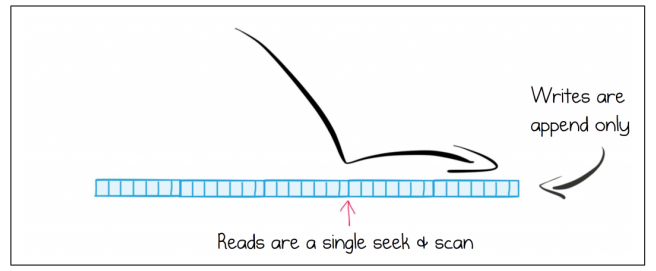
\includegraphics[scale=0.8]{figure4.1.png}
    Figura 4-1\\
    -Extracto del libro 'Designing Event-Driven Systems' por Ben Stopford, publicado por O'Reilly Media, Inc. Copyright © 2018 O'Reilly Media. Todos los derechos reservados.-
\end{center}
La adopción de un enfoque log-estructurado tiene un efecto interesante. Tanto las lecturas como las escrituras son operaciones secuenciales. Esto las hace afines a la medio subyacente, aprovechando el pre-fetch, las diferentes capas de caché y agrupando naturalmente las operaciones. Esto a su vez las hace eficientes. De hecho, cuando se leen mensajes de Kafka, el servidor ni siquiera los importa en la Máquina Virtual de Java. Los datos se copian directamente del búfer del disco al búfer de la red (zero copy), una oportunidad que brinda la simplicidad tanto del contrato como de la estructura de datos subyacente.\\

Por lo tanto, las operaciones secuenciales agrupadas ayudan con el rendimiento general. También hacen que el sistema sea adecuado para almacenar mensajes a largo plazo. La mayoría de los intermediarios de mensajería tradicionales están construidos con estructuras de índice: tablas hash o árboles B- utilizados para administrar los reconocimientos, filtrar los encabezados de los mensajes y eliminar los mensajes cuando han sido leídos. Pero la desventaja es que estos índices deben mantenerse, y esto tiene un costo. Deben mantenerse en la memoria para obtener un buen rendimiento, limitando significativamente la retención. Pero el log es O(1) tanto al leer como al escribir mensajes en una partición, por lo que importa poco si los datos están en el disco o están en caché en la memoria.\\

Hay algunas implicaciones de este enfoque log-estructurado. Si un servicio tiene algún tipo de interrupción y no lee mensajes por un largo período de tiempo, el acúmulo no causará que la infraestructura se ralentice significativamente (un problema común con los intermediarios tradicionales, que tienden a ralentizarse a medida que se llenan). Al ser log-estructurado, Kafka también es adecuado para desempeñar el papel de un almacén de eventos, para aquellos que deseen aplicar el almacenamiento de eventos dentro de sus servicios.

\subsection{Particiones y compartimentación}
El concepto de particiones es fundamental para la mayoría de los sistemas de datos distribuidos. Una partición es simplemente un recipiente en el que se coloca datos, al igual que los recipientes que se utilizan para agrupar datos en una tabla hash. En el terminología de Kafka, cada registro es una réplica de una partición que se almacena en una máquina diferente. (Por lo tanto, una partición puede tener tres réplicas para garantizar alta disponibilidad. Cada réplica es un registro separado con los mismos datos en su interior.) Lo que se coloca en cada partición se determina por un particionador, codificado en el productor de Kafka. El particionador difundirá los datos de manera equilibrada entre las particiones disponibles en una rotación o, si se proporciona una clave con el mensaje, usará un hash de la clave para determinar el número de partición. Este último punto garantiza que los mensajes con la misma clave siempre se envíen a la misma partición y, por lo tanto, están fuertemente ordenados.

\subsection{Escalabilidad lineal}
 La escalabilidad lineal en Kafka se logra a través del uso de múltiples registros distribuidos en múltiples máquinas. Este conjunto garantiza que los mensajes se encaminen y se repliquen de manera confiable para garantizar la tolerancia a fallos y que el sistema pueda manejar fallos de manera adecuada. Los registros proporcionan una estructura de datos eficiente para las cargas de trabajo de mensajería y están optimizados para el hardware subyacente. Aunque es posible ejecutar Kafka en una sola máquina, los clústeres de producción típicamente consisten en tres o más máquinas, con clústeres más grandes que alcanzan cientos de máquinas. Al acceder a un tópico para lectura o escritura, se accede a todas las máquinas del clúster. Para escalar el sistema, simplemente puede agregar más máquinas y reequilibrar los datos. Además, la consumición de mensajes se puede realizar en paralelo, con mensajes de un tópico distribuidos entre múltiples consumidores en un grupo de consumidores.

\begin{center}
    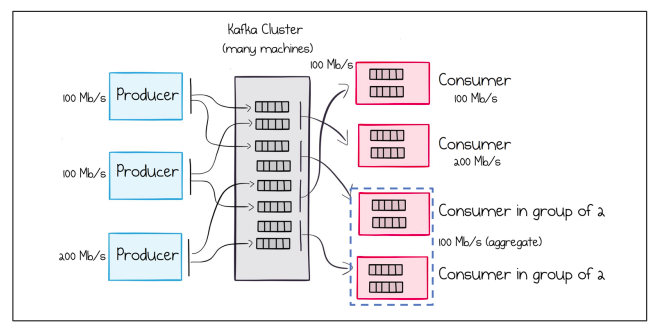
\includegraphics[scale=0.8]{figure4.2.png}
    Figura 4-2\\
    -Extracto del libro 'Designing Event-Driven Systems' por Ben Stopford, publicado por O'Reilly Media, Inc. Copyright © 2018 O'Reilly Media. Todos los derechos reservados.-
\end{center}

El principal avantage de esto, desde una perspectiva arquitectónica, es que quita la problemática de escalabilidad de la mesa. Con Kafka, es virtualmente imposible alcanzar una barrera de escalabilidad en el contexto de sistemas empresariales. Esto puede ser muy empoderador, especialmente cuando los ecosistemas crecen, permitiendo a los implementadores elegir patrones que son un poco más libres con el ancho de banda y el movimiento de datos.\\

La escalabilidad también abre otras oportunidades. Clústeres únicos pueden crecer a escala empresarial, sin el riesgo de que las cargas de trabajo sobrepoten a la infraestructura. Por ejemplo, New Relic se basa en un solo clúster de alrededor de 100 nodos, que abarca tres centros de datos y procesa 30 GB/s. En otros dominios menos intensivos en datos, clústeres de 5 a 10 nodos comúnmente soportan cargas de trabajo de toda la empresa. Pero debemos tener en cuenta que no todas las empresas eligen la ruta de -un solo gran clúster-. Por ejemplo, Netflix aconseja usar varios clústeres más pequeños para reducir los costos operativos de ejecutar instalaciones muy grandes, pero su instalación más grande aún está alrededor de la marca de 200 nodos.\\

Para administrar clústeres compartidos, es útil dividir el ancho de banda, utilizando las características de segregación de ancho de banda que vienen con Kafka. Hablaremos sobre ellos a continuación.

\subsection{Segregación de la carga en ecosistemas multiservicio}
Kafka ha sido diseñado para ser utilizado por múltiples servicios, convirtiéndolo en un sistema multitenant. En muchas empresas, todos los servicios comparten un único clúster de producción, pero esto también aumenta el riesgo de ataques accidentales de denegación de servicio que podrían llevar a una degradación o inestabilidad del servicio. Para mitigar este riesgo, Kafka incluye una característica llamada cuotas, que permite a los administradores asignar una cantidad específica de ancho de banda a cada servicio, asegurándose de que opera dentro de los acuerdos de nivel de servicio definidos. Esta característica ayuda a prevenir la competencia de red inesperada, ya que los servicios codiciosos son fuertemente limitados, permitiendo que un único clúster sea utilizado por muchos servicios sin temor a problemas de rendimiento. Las cuotas se pueden aplicar a instancias de servicios individuales o grupos que estén equilibrados de carga.

\subsection{Mantener sólidas garantías de pedido}
Además, es importante considerar que los mensajes deben ser escritos y leídos en el mismo orden en el que fueron producidos. Esto significa que los productores deben escribir los mensajes en un orden estricto antes de enviarlos a los consumidores. Los consumidores deben leer los mensajes en el orden en que fueron producidos, respetando la secuencia. Para lograr esto, Kafka utiliza una estructura de datos llamada cola de mensajes, que permite a los productores escribir mensajes en un orden específico y a los consumidores leerlos en el mismo orden. En resumen, para garantizar garantías de orden fuerte, los mensajes deben ser escritos y leídos en un orden específico y deben ser enrutados al mismo partición, utilizando la misma clave para los mensajes relacionados.
\begin{center}
    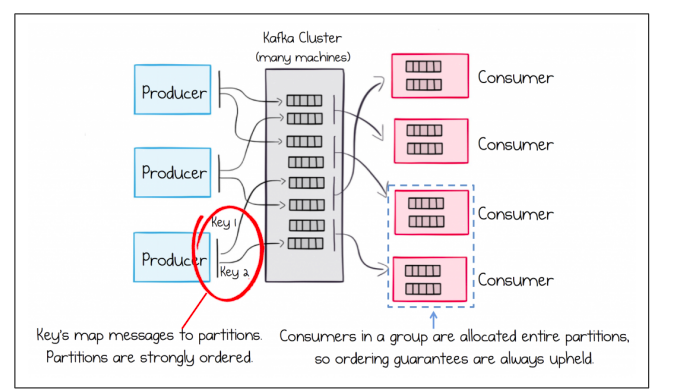
\includegraphics[scale=0.8]{figure4.3.png}
    Figura 4-3\\
    -Extracto del libro 'Designing Event-Driven Systems' por Ben Stopford, publicado por O'Reilly Media, Inc. Copyright © 2018 O'Reilly Media. Todos los derechos reservados.-
\end{center}
Además, para garantizar garantías de orden fuerte, es importante tener en cuenta los reintentos. En la mayoría de los casos, queremos habilitar los reintentos en el productor para que, en caso de algún problema en la red, recolección de basura de larga duración, fallo o similares, cualquier mensaje que no se haya enviado con éxito al clúster se vuelva a intentar. La sutileza es que los mensajes se envían en lotes, por lo que debemos tener cuidado de enviar estos lotes uno por una vez, por máquina de destino, para que no haya una posibilidad de reordenamiento de eventos cuando ocurran fallos y se reintente los lotes. Esto es simplemente algo que configuramos.
\subsection{Garantizar la durabilidad de los mensajes}
Kafka asegura la durabilidad a través de la replicación. Esto significa que los mensajes son escritos en un número configurable de máquinas de tal manera que si una o más de esas máquinas fallan, los mensajes no se perderán. Si configura un factor de replicación de tres, dos máquinas pueden fallar sin perder datos.\\

Para aprovechar al máximo la replicación, para conjuntos de datos sensibles como los que se ven en las aplicaciones basadas en servicios, configure tres réplicas para cada partición y configure el productor para esperar que se complete la replicación antes de continuar. Finalmente, como se discutió anteriormente, configure las reintentos en el productor.\\

En aplicaciones altamente sensibles, es posible que sea necesario que los datos se escriban en disco de forma sincrónica para garantizar la integridad de los datos. Sin embargo, esta abordaje debe utilizarse con moderación, ya que tendrá un impacto significativo en el rendimiento, especialmente en entornos altamente concurrentes. Si se opta por esta opción, se recomienda aumentar el tamaño del lote del productor para aumentar la efectividad de cada escritura en disco en la máquina (los mensajes se escriben en disco juntos en forma de lote). Este enfoque también es útil en implementaciones en una sola máquina, donde se ejecuta un solo nodo ZooKeeper en la misma máquina y los mensajes se escriben en disco de forma sincrónica para asegurar la resiliencia.
\subsection{Servicios de equilibrio de carga y hacerlos altamente disponibles}
Además, es importante asegurarse de que el balanceo de carga se realice de manera efectiva y equilibrada entre los servicios. Esto se puede lograr configurando múltiples instancias de un servicio y permitiendo que Kafka asigne las particiones de manera equilibrada entre ellas. De esta manera, se asegura que la carga se distribuya entre las instancias y se brinde alta disponibilidad en caso de fallo de un nodo.
\begin{center}
    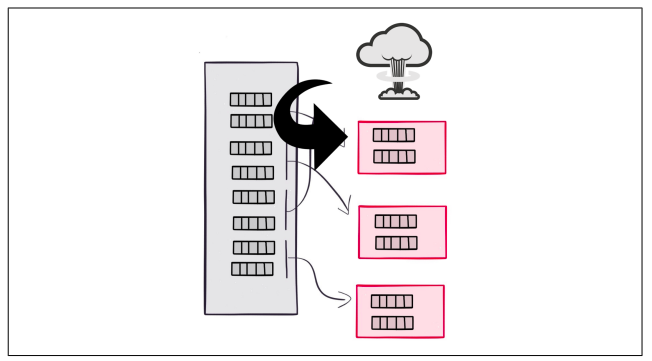
\includegraphics[scale=0.8]{figure4.4.png}
    Figura 4-4\\
    -Extracto del libro 'Designing Event-Driven Systems' por Ben Stopford, publicado por O'Reilly Media, Inc. Copyright © 2018 O'Reilly Media. Todos los derechos reservados.-
\end{center}
Este proceso funciona asignando enteras particiones a diferentes consumidores. Una de las fortalezas de esta aproximación es que una sola partición solo puede ser asignada a una única instancia de servicio (consumidor). Esto es un invariante, lo que implica que la ordenación está garantizada, incluso cuando los servicios fallan y se reinician.\\

De esta manera, los servicios heredan tanto la disponibilidad alta como el equilibrio de carga, lo que significa que pueden escalar, manejar interrupciones imprevistas o realizar reinicios sucesivos sin interrupciones en el servicio. De hecho, las liberaciones de Kafka siempre son compatibles con la versión anterior, por lo que se garantiza poder liberar una nueva versión sin tener que detener el sistema.

\subsection{Temas compactados}
Por defecto, los temas en Kafka son basados en retención: los mensajes se retienen por cierto
tiempo configurable. Kafka también incluye un tipo especial de tema que
administra conjuntos de datos con clave, es decir, datos que tienen una clave principal (identificador) como puede tener en una tabla de base de datos. Estos temas compactados solo retienen los eventos más recientes, con cualquier evento antiguo, para una cierta clave, que se eliminan. También admiten eliminaciones.
Los temas compactados funcionan un poco como árboles LSM simples (log-structure merge-trees).\\

El tema se escanea periódicamente y se eliminan los mensajes antiguos si han sido reemplazados (basados en su clave); ver la figura 4-5. Vale la pena señalar que este es
un proceso asíncrono, por lo que un tema compactado puede contener algunos mensajes reemplazados, que están esperando ser comprimidos.
\begin{center}
    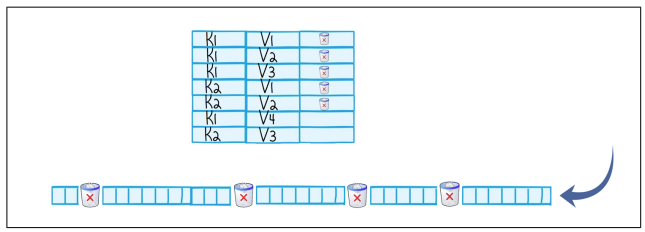
\includegraphics[scale=0.8]{figure4.5.png}
    Figura 4-5\\
    -Extracto del libro 'Designing Event-Driven Systems' por Ben Stopford, publicado por O'Reilly Media, Inc. Copyright © 2018 O'Reilly Media. Todos los derechos reservados.-
\end{center}

Los tópicos compactados permiten hacer un par de optimizaciones. En primer lugar, nos ayudan a ralentizar el crecimiento de un conjunto de datos (eliminando eventos superados), pero lo hacemos de una manera específica para los datos en lugar de, por ejemplo, simplemente eliminar mensajes más antiguos de dos semanas. En segundo lugar, tener conjuntos de datos más pequeños nos resulta más fácil moverlos de una máquina a otra.\\

Los tópicos compactados permiten hacer un par de optimizaciones. Primero, ayudan a reducir el crecimiento de un conjunto de datos (eliminando eventos reemplazados), pero lo hacemos de una manera específica para los datos en lugar de, por ejemplo, simplemente eliminar mensajes antiguos de hace dos semanas. Segundo, tener conjuntos de datos más pequeños hace más fácil moverlos de una máquina a otra.\\

Esto es importante para el procesamiento en flujo con estado. Digamos que un servicio usa la API de Streams de Kafka para cargar la última versión del catálogo de productos en una tabla (como se discutió en -Ventanas, Uniones, Tablas y Tiendas de Estado- en la página 139 del Capítulo 14, una tabla es una tabla hash residente en el disco dentro de la API). Si el catálogo de productos se almacena en un tópico compactado en Kafka, la carga se puede realizar más rápido y eficientemente si no tiene que cargar toda la historia versionada (como sería el caso con un tópico regular).

\subsection{Almacenamiento de datos a largo plazo}
Una de las diferencias más grandes entre Kafka y otros sistemas de mensajería es que
se puede utilizar como una capa de almacenamiento. De hecho, no es raro ver tópicos
basados en retención o tópicos compactados que contienen más de 100 TB de datos. Pero Kafka no es una
base de datos; es un registro de compromisos que no ofrece funcionalidad de consulta amplia (y no hay
planes para que esto cambie). Pero su contrato simple resulta bastante útil
para almacenar conjuntos de datos compartidos en sistemas grandes o arquitecturas de la empresa, por ejemplo, el uso de eventos como una fuente compartida de verdad.\\

Los datos se pueden almacenar en tópicos regulares, que son excelentes para auditoría o Event Sourcing,
o tópicos compactados, que reducen el perfil general. Puede combinar los
dos, obteniendo lo mejor de ambos mundos a un precio adicional de almacenamiento, manteniendo
ambos y vinculándolos juntos con un trabajo de Kafka Streams. Este patrón se llama
el patrón de versión más reciente.

\subsection{Seguridad}
Kafka proporciona una serie de características de seguridad de grado empresarial para la autenticación y autorización. La autenticación del cliente se proporciona a través de Kerberos o certificados TLS de cliente, garantizando que el clúster de Kafka conozca quién está haciendo cada solicitud. También hay un sistema de permisos similar a Unix, que se puede utilizar para controlar qué usuarios pueden acceder a qué datos. La comunicación de red se puede cifrar, lo que permite enviar mensajes de forma segura a través de redes no confiables. Finalmente, los administradores pueden requerir autenticación para la comunicación entre Kafka y ZooKeeper.\\

El mecanismo de cuotas, discutido en la sección -Segregación de la carga en ecosistemas de múltiples servicios- en la página 21, se puede vincular a esta noción de identidad, y las características de seguridad de Kafka se extienden a través de los diferentes componentes de la plataforma Confluent (Rest Proxy, Confluent Schema Registry, Replicator, etc.).

\subsection{Resumen}
En resumen, Kafka es un poco diferente a la tecnología de mensajería promedio. Al ser diseñado como un componente de infraestructura distribuido y escalable, lo convierte en un hueso ideal a través del cual los servicios pueden intercambiar y almacenar temporalmente eventos. Obviamente, hay una serie de elementos únicos de la tecnología en sí, pero los que sobresalen son sus capacidades para escalar, funcionar siempre y retener conjuntos de datos a largo plazo.\\

Podemos usar los patrones y características discutidos en este capítulo para construir una amplia variedad de arquitecturas, desde sistemas finamente granulados basados en servicios hasta conglomerados corporativos masivos. Este es un enfoque seguro, pragmático y probado y comprobado.

\newpage
\section{Ejemplo práctico de kafka}
\subsection{Instalación}
instalaremos Apache kafka en Ubuntu.
\subsubsection{Instalación del jdk}
Para realizar la instalación del jdk en ubuntu se puede realizar por medio de la terminal (abrir con ctrl + alt + T)\\
En la terminal de ubuntu digitamos los siguientes comandos:
\begin{itemize}
    \item \begin{lstlisting}[numbers=none]
sudo apt update\end{lstlisting}
Nos sirve para actualizar la lista de paquetes disponibles y sus versiones.
    \item \begin{lstlisting}[numbers=none]
sudo apt install default-jdk\end{lstlisting}
Nos instalará el jdk por defecto. (NOTA: El segundo comando puede ser modificado para hacer la instalación del jdk que desees, por defecto se instalará la última versión.
\end{itemize}
Puedes ver que la instalación fue exitosa ejecutando el comando:
\begin{lstlisting}[numbers=none]
    java --version\end{lstlisting}
Y el resultado será algo similar a:
\begin{lstlisting}[numbers=none]
    openjdk 11.0.17 2022-10-18
    OpenJDK Runtime Environment (build 11.0.17+8-post-Ubuntu-1ubuntu2)\end{lstlisting}
\subsubsection{Instalación Apache Kafka}
Asegurate de estar en la carpeta downloads antes de ejecutar el siguiente comando, desde la terminal con el comando:
\begin{lstlisting}[numbers=none]
    wget https://dlcdn.apache.org/kafka/3.2.0/kafka_2.13-3.2.0.tgz\end{lstlisting}
Una vez descargado el .tgz de kafka nos vamos a downloads, abrimos una terminal y descomprimimos el archivo con el comando:
\begin{lstlisting}[numbers=none]
    tar xzf kafka_2.13-3.2.0.tgz \end{lstlisting}
y movemos la carpeta descomprimida al directorio /usr/local con el comando:
\begin{lstlisting}[numbers=none]
    sudo mv kafka-3.4.0-src /usr/local/kafka\end{lstlisting}
\subsubsection{Iniciar el apache kafka}
Para iniciar el apache kafka hay que ir a la carpeta de kafka en usr/local/kafka y ejecutando el siguiente comando:
\begin{lstlisting}[numbers=none]
    bin/zookeeper-server-start.sh config/zookeeper.properties\end{lstlisting}
Para iniciar el servidor de kafka hay que abrir una nueva terminal en la carpeta /usr/local/kafka y ejecutamos el comando:
\begin{lstlisting}[numbers=none]
    bin/kafka-server-start.sh config/server.properties\end{lstlisting}
Una vez creado los archivos zookeeper.service y kafka.service debemos reiniciar el sytemd daemon para poder guardar los cambios a los archivos usando el comando:
\begin{lstlisting}[numbers=none]
    systemctl daemon-reload\end{lstlisting}
Después de realizar esto se puede iniciar el zookeeper y el apache kafka con los comandos.
\begin{lstlisting}[numbers=none]
    sudo systemctl start zookeeper\end{lstlisting}
y
\begin{lstlisting}[numbers=none]
    sudo systemctl start kafka\end{lstlisting}
Y ya se puede usar zookeeper y apache kafka.

\subsection{Creación y listado de topics }
Para poder crear topics y listarlos se debe abrir una terminal e ir hasta la carpeta donde movimos los archivos de kafka, una vez ahí ejecutamos el siguiente comando para listar los topics creados (NOTA: Previamente se deben arrancar el zookeeper y el servidor de kafka)  (si no hay algún topic creado, no debe aparecer nada). 
\begin{lstlisting}[numbers=none]
    bin/kafka-topics.sh --list --bootstrap-server localhost:9092\end{lstlisting}
Con este comando usamos el script kafka-topics para listar todos los topics que hemos creado, especificando la url del servidor de zookeeper que se encarga de la administración de los topics, el resultado de este comando es:
\begin{lstlisting}[numbers=none]
    test-topic\end{lstlisting}

Para la creación de topics se hace uso del mismo script y se utilizará el siguiente comando.\\
{\tiny 
\begin{lstlisting}[numbers=none]
        bin/kafka-topics.sh --create --topic test-topic --bootstrap-server localhost:9092 --replication-factor1 --partitions 1\end{lstlisting} }
En este comando damos la orden de crear, especificamos el nombre del topic, la url donde se encuentra en ejecución el zookeeper, el factor de replicación y finalmente el número de particiones del topic, el resultado es:
\begin{lstlisting}[numbers=none]
    Created topic test-topic.\end{lstlisting}
Otras opciones que podemos encontrar son alter y describe, para modificar topics y ver los detalles de un topic en específico
\subsection{Publicar contenido en un topic con un productor por terminal}
Para este caso podemos usar el mismo topic que creamos anteriormente y la misma terminal, ejecutamos el comando que nos permite abrir el productor el cual es el siguiente:
\begin{lstlisting}[numbers=none]
    bin/kafka-console-producer.sh --broker-list localhost:9092 --topic testTopic\end{lstlisting}
Haciendo uso del script kafka-console-producer.sh especificamos el cluster de kafka donde se encuentran los broker y el nombre del topic en el que queremos poner un mensaje, al ejecutarlo podremos escribir los mensajes y así se ve:
\begin{lstlisting}[numbers=none]
    >Hola
    >Esto es un mensaje de prueba\end{lstlisting}
En este ejemplo escribimos 2 mensajes en el topic test Topic, Hola y Esto es un mensaje de prueba.
\subsection{Consumir datos de un topic con un consumidor por terminal}
Para este caso podemos hacer uso de la misma terminal saliendo del productor con ctrl + c y luego ejecutaremos el comando para abrir un consumidor, el comando es:
\begin{lstlisting}[numbers=none]
    bin/kafka-console-consumer.sh --bootstrap-server localhost:9092 --topic testTopic --from-beginning\end{lstlisting}
Se especifican los host desde donde leeremos los mensajes el topic y el --from-beginning permite traer todos los mensajes del topic que estén almacenados, en este caso se verán los 2 mensajes anteriores que creamos con el productor
\begin{lstlisting}[numbers=none]
    Hola
    Esto es un mensaje de prueba\end{lstlisting}
Como se evidencia los mensajes antes publicados en el productor pudimos obtenerlos en el consumidor sin problema alguno, si se abren terminales diferentes para el consumidor y productor se podrá ver que los mensajes escritos en el productor se reflejan en el consumidor en tiempo real.

\subsection{Mensajes con key}
Otra opción para enviar mensajes es especificando un key para el mensaje, en este caso se deben agregar a los comandos para ejecutar el productor y el consumidor las propiedades para describir que el mensaje tendrá un key, en caso de no hacerlo el key es null por defecto, las propiedades para junto con el comando se describen a continuación:
\begin{lstlisting}[numbers=none]
    -property parse.key=true --property key.separator=:\end{lstlisting}
Se especifica que el key será requerido y que el separador del key y el mensaje será:\\
Productor:
\begin{lstlisting}[numbers=none]
    bin/kafka-console-producer.sh --broker-list localhost:9092 --topic testTopic --property parse.key=true --property key.separator=:\end{lstlisting}
Consumidor:\\
    \begin{lstlisting}[numbers=none]
    bin/kafka-console-consumer.sh --bootstrap-server localhost:9092 --topic testTopic --from-beginning --property print.key=true --property key.separator=:\end{lstlisting}
Estos son los resultados:
\begin{lstlisting}[numbers=none]
    Esto es un mensaje de prueba
    Este es el lado del productor
    Desde el productor escribimos al consumidor
    -El consumidor puede responder
    Pero el productor no recibe mensajes de este lado
    El consumidor puede observar todos los mensajes del productor\end{lstlisting}
Así se generan mensajes desde el terminal especificando el key, como podemos ver para los mensajes anteriores donde no se especificó el key el consumidor todo el key como null.
\subsection{Ejercicios}
\begin{ejercicio}
    Crear, listar y describir topics.\\
    \sol
    Para crear, listar y describir tópicos en Apache Kafka, puedes utilizar los siguientes comandos:
    \begin{itemize}
        \item Crear tópico:\\
            Para crear un tópico en Apache Kafka, puedes utilizar el siguiente comando:\\
            \texttt{bin/kafka-topics.sh --create --topic name-topic --bootstrap-server localhost:9092 --replication-factor 1 --partitions 1}
        \item Listar tópicos:\\
            Para listar todos los tópicos existentes en Apache Kafka, puedes utilizar el siguiente comando:
            \texttt{/bin/kafka-topics.sh --list --bootstrap-server localhost:9092}\\
            El resultado:
\begin{lstlisting}[numbers=none]
    name-topic
    test-topic
    testTopic\end{lstlisting}
        \item Describir tópico:\\
            Para describir un tópico en particular en Apache Kafka, puedes utilizar el siguiente comando:\\
            \texttt{bin/kafka-topics.sh --describe --bootstrap-server localhost:9092 --topic name-topic}\\
            El resultado:
            \end{itemize}
            {\scriptsize
\begin{lstlisting}[numbers=none]
    Topic: name-topic	TopicId: mmK6zBn3RCWi-vbJ9YIe-Q	PartitionCount: 1	ReplicationFactor: 1	Configs  segment.bytes=1073741824
       Topic: name-topic	Partition: 0	Leader: 0	              Replicas: 0	Isr: 0 \end{lstlisting}}
\end{ejercicio}
\begin{ejercicio}
    Crear Productor para un topic por consola.\\
    \sol
    \begin{itemize}
        \item Para crear un productor para un topic por consola, puedes usar el siguiente comando en la línea de comandos:
        \begin{lstlisting}[numbers=none]
            bin/kafka-console-producer.sh --broker-list localhost:9092 --topic name-topic\end{lstlisting}
        nos despliega un menú donde se puede empezar a escribir como el \textbf{productor}\\
        Resultados:
        \end{itemize}
\begin{lstlisting}[numbers=none]
    >Hola este es el productor de name-topic
\end{lstlisting}
\end{ejercicio}
\begin{ejercicio}
    Crear Consumidor para un topic por consola.\\
    \sol
    \begin{itemize}
        \item Para crear un consumidor de un topic en la consola, primero debes iniciar una sesión de la línea de comandos en tu servidor donde está instalado Apache Kafka.
        \begin{lstlisting}[numbers=none]
            bin/kafka-console-consumer.sh --bootstrap-server localhost:9092 --topic name-topic --from-beginning\end{lstlisting}
        nos despliega un menú donde se puede empezar a leer como el \textbf{Consumidor}\\
        Resultados:        
    \end{itemize}
    \begin{lstlisting}[numbers=none]
    Hola este es el productor de name-topic
\end{lstlisting}
\end{ejercicio}
\begin{ejercicio}
    Crear Productor con key por consola.\\
    \sol
    \begin{itemize}
        \item
        \begin{lstlisting}[numbers=none]
           bin/kafka-console-producer.sh --broker-list localhost:9092 --topic name-topic --property parse.key=true --property key.separator=:\end{lstlisting}
    \end{itemize}
\end{ejercicio}
\begin{ejercicio}
    Crear Consumidor con key por consola.\\
    \sol
    \begin{itemize}
        \item
        \begin{lstlisting}[numbers=none]
            bin/kafka-console-producer.sh --broker-list localhost:9092 --topic name-opic --property parse.key=true --property key.separator=:\end{lstlisting}
    \end{itemize}
\end{ejercicio}

\newpage
\section{Docker}
 Docker es una plataforma de software que permite a los desarrolladores empaquetar y distribuir sus aplicaciones en contenedores. Un contenedor es una unidad estandarizada de software que incluye todo lo necesario para ejecutar una aplicación, como el código, las bibliotecas y las dependencias. Docker te permite crear imágenes de tus aplicaciones y ejecutarlas en cualquier entorno que tenga Docker instalado.

 \subsection{instalación de Docker}
 para instalar Docker en linux hay que seguir los siguientes pasos:
 \begin{enumerate}
     \item Abre una terminal en tu sistema operativo Ubuntu.
     \item Actualiza el índice de paquetes de apt:
     \begin{lstlisting}[numbers=none]
         sudo apt-get update\end{lstlisting}
     \item Instala los paquetes necesarios para permitir a apt usar un repositorio sobre HTTPS:
\begin{lstlisting}[numbers=none]
 sudo apt-get install apt-transport-https ca-certificates curl gnupg lsb-release \end{lstlisting}
     \item Agrega la clave GPG oficial de Docker:
\begin{lstlisting}[numbers=none]
curl -fsSL https://download.docker.com/linux/ubuntu/gpg | sudo gpg --dearmor -o /usr/share/keyrings/docker-archive-keyring.gpg   \end{lstlisting}
     \item Usa el siguiente comando para configurar el repositorio estable de Docker:
 \begin{lstlisting}[numbers=none]
 echo -deb [arch=amd64 signed-by=/usr/share/keyrings/docker-archive-keyring.gpg] https://download.docker.com/linux/ubuntu \
(lsb_release -cs) stable- | sudo tee /etc/apt/sources.list.d/docker.list > /dev/null\end{lstlisting}
     \item Actualiza el índice de paquetes de apt:
 \begin{lstlisting}[numbers=none]
 sudo apt-get update\end{lstlisting}
 \item Finalmente, instala Docker:
 \begin{lstlisting}[numbers=none]
 sudo apt-get install docker-ce docker-ce-cli containerd.io    \end{lstlisting}
\end{enumerate}
Una vez que la instalación haya finalizado, ya deberías poder usar Docker. Puedes probarlo ejecutando el siguiente comando:
 \begin{lstlisting}[numbers=none]
    sudo docker run hello-world\end{lstlisting}
Este comando descarga una imagen de prueba de Docker y la ejecuta en un contenedor. Si todo funciona bien, verás un mensaje de prueba en tu terminal.\\

Recuerda que si estás usando un sistema operativo distinto a Ubuntu, los pasos pueden variar.
\subsection{Creación de un Dockerfile}
\begin{enumerate}
\item\textbf{construimos una carpeta}\\ 
     Vamos a crear una carpeta llamada dockerweb en HOME asi
\begin{lstlisting}[numbers=none]
    mkdir ~/dockerweb/\end{lstlisting}
\item \textbf{Creamos un archivo Dockerfile}\\ 
     El Dockerfile es un archivo de texto que contiene las instrucciones para construir una imagen de Docker. Creamos un archivo llamado Dockerfile asi:
\begin{lstlisting}[numbers=none]
    nano ~/dockerweb/Dockerfile\end{lstlisting}
    \item \textbf{Escribimos el Dockerfile}\\ 
    en el editor que se abrió después del comando anterior escribimos
    \begin{lstlisting}[numbers=none]
    Contenido de Dockerfile
    FROM ubuntu:latest
    MAINTAINER KEVIN kevin.cardenas1@quind.io
    RUN apt-get update
    RUN apt-get -y install apache2
    expose 80
    CMD /usr/sbin/apache2ctl -D FOREGROUND\end{lstlisting}
    \item \textbf{Ejecución del Dockerfle} \\ 
    Ejecutamos en docker el contenido de Dockerfile asi:
    \begin{lstlisting}[numbers=none]
    sudo docker build -t web ~/dockerweb/\end{lstlisting}
    \item Si miramos nuestras imágenes de docker vamos a ver una nueva llamada web.
    \begin{lstlisting}[numbers=none]
    sudo docker images\end{lstlisting}
    \item \textbf{Creación del contenedor}\\ 
     Una vez que se ha creado el Dockerfile, se puede construir la imagen utilizando el siguiente comando en la línea de comandos:
    Ejecutamos en docker el contenido de Dockerfile asi:
    \begin{lstlisting}[numbers=none]
    sudo docker run -d -p 8085:80 web\end{lstlisting}
    Donde:
    -d : Corre el contenedor en background.\\
    -p 8085:80 : Lee el puerto 80 del contenedor y lo corre en el puerto 8085 de la maquina anfitrion.\\
    web : Nombre de la imagen a correr.
    \item \textbf{Inicio del contenedor:}\\ 
    Después de construir la imagen, se puede iniciar un contenedor utilizando la siguiente línea de comandos:
    \begin{lstlisting}[numbers=none]
    sudo docker run -d -p 8085:80 web\end{lstlisting}
    \item \textbf{listar los contenedores}\\ 
    Para listar los contenedores, utilice el siguiente comando:
    \begin{lstlisting}[numbers=none]
    sudo docker ps\end{lstlisting}
    \item \textbf{Verificación de los logs:}\\
    Para ver los logs de un contenedor en ejecución, utilice el siguiente comando:
    \begin{lstlisting}[numbers=none]
    docker logs <container_id>\end{lstlisting}
    \item puedes ver el puerto entrando a \href{http://localhost:8085/}{localhost:8085}
    \item \textbf{Detener y eliminar el contenedor:}\\ 
    Para detener un contenedor en ejecución, utilice el siguiente comando:
    \begin{lstlisting}[numbers=none]
    docker stop <container_id>\end{lstlisting}
    Para eliminar un contenedor detenido, utilice el siguiente comando:
    \begin{lstlisting}[numbers=none]
    docker rm <container_id>\end{lstlisting}
\end{enumerate}
Estos son solo los comandos básicos de Docker, hay muchos otros comandos y características disponibles para manejar contenedores y imágenes.\\

\subsection{Crear una imagen de Docker a partir de un Dockerfile}

Para crear una imagen de Docker a partir de un Dockerfile, sigue estos pasos:

\begin{enumerate}
\item Crea un archivo llamado \lstinline{Dockerfile} en el directorio de trabajo actual.
\item Agrega el siguiente contenido al archivo Dockerfile:

\begin{lstlisting}[numbers=none]
FROM python:3.7-alpine
WORKDIR /app
COPY . /app
RUN pip install -r requirements.txt
CMD [-python-, -app.py-]
\end{lstlisting}
\item Crea una imagen de Docker ejecutando el siguiente comando: \lstinline{docker build -t myapp .}
\item Ejecuta un contenedor de la imagen que acabas de crear: \lstinline{docker run -p 5000:5000 myapp}
\item Abre un navegador web y navega a \lstinline{http://localhost:5000}. Verás la aplicación web que acabas de crear.
\end{enumerate}

\newpage
\section{Kafka connect}
Kafka Connect es un framework para conectar aplicaciones externas con Apache Kafka. Proporciona una manera de transferir datos de manera fácil, escalable y confiable desde sistemas externos a Kafka o desde Kafka a sistemas externos. Los usuarios pueden definir las conexiones mediante una configuración simple y los datos se transfieren automáticamente, sin la necesidad de programación adicional. Esto hace que sea ideal para la integración de datos en el entorno de big data de Apache Kafka.\\

Kafka Connect es como un puente que conecta diferentes sistemas y permite la transferencia de datos entre ellos de forma confiable y escalable. Al igual que un puente conecta dos orillas, Kafka Connect conecta dos sistemas y permite que los datos fluyan entre ellos. Con Kafka Connect, puedes transferir datos desde diferentes fuentes, como bases de datos, aplicaciones, sistemas de archivos, y otros, a Kafka, y luego distribuir estos datos a diferentes destinos, como aplicaciones, bases de datos, y otros.
\subsection{Hacer quickstar de kafka connect Quickstart}
Para hacer un quickstart de Apache Kafka Connect, primero debes tener Apache Kafka y Apache ZooKeeper instalados y en ejecución en tu sistema. Si no los tienes instalados, puedes descargarlos de la página oficial de Apache Kafka.\\
A continuación, seguimos los siguientes pasos:
\begin{itemize}
    \item \textbf{Inicia Apache ZooKeeper:}
    \begin{lstlisting}[numbers=none]
bin/zookeeper-server-start.sh config/zookeeper.properties\end{lstlisting}
    \item \textbf{Inicia Apache Kafka:}
    \begin{lstlisting}[numbers=none]
bin/kafka-server-start.sh config/server.properties\end{lstlisting}
    \item \textbf{Crea un topic de prueba:}
    \begin{lstlisting}[numbers=none]
bin/kafka-topics.sh --create --bootstrap-server localhost:9092 --replication-factor 1 --partitions 1 --topic test\end{lstlisting}
    \item \textbf{Inicia Apache Kafka Connect:}
    \begin{lstlisting}[numbers=none]
bin/connect-standalone.sh config/connect-standalone.properties\end{lstlisting}
    \item \textbf{Crea un archivo de configuración de plugin para un conector de archivos de texto:}
    \begin{lstlisting}[numbers=none]
name=local-file-sink
connector.class=FileStreamSink
tasks.max=1
topics=test
file=test.txt\end{lstlisting}
    \item \textbf{Envía algunos mensajes a tu topic de prueba:}
    \begin{lstlisting}[numbers=none]
bin/kafka-console-producer.sh --broker-list localhost:9092 --topic test\end{lstlisting}
    \item Verifica los archivos de logs de Apache Kafka Connect y deberías ver los mensajes que enviaste a tu topic de prueba.
    \item \textbf{Detén Apache Kafka Connect y Apache Kafka}.\\
    Utiliza el siguiente comando para detener la ejecución de Apache Kafka Connect:
    \begin{lstlisting}[numbers=none]
bin/connect-standalone.sh stop\end{lstlisting}
Verifica que Apache Kafka Connect ya no esté ejecutándose utilizando el siguiente comando:
    \begin{lstlisting}[numbers=none]
ps aux | grep connect\end{lstlisting}
    Si Apache Kafka Connect ya no aparece en la lista de procesos en ejecución, significa que ha sido detenido correctamente.
\end{itemize}
\subsubsection{Hacer un quickstart de Kafka Connect}

Kafka Connect es una herramienta para conectar fuentes de datos externas a Kafka. Con Kafka Connect, puedes leer datos de una variedad de fuentes, como bases de datos, sistemas de archivos y aplicaciones web, y escribirlos en Kafka. También puedes leer datos de Kafka y escribirlos en una variedad de destinos.

Para hacer un quickstart de Kafka Connect, sigue los siguientes pasos:

\begin{enumerate}
\item Descarga la versión de Kafka que deseas utilizar desde el sitio web de Apache Kafka y descomprímela en tu sistema.
\item Configura el archivo de configuración de Kafka. En el directorio de Kafka, encuentra el archivo de configuración \lstinline{config/server.properties} y configúralo según tus necesidades. Asegúrate de configurar correctamente las propiedades \lstinline{advertised.listeners} y \lstinline{listeners} para que Kafka pueda escuchar las conexiones entrantes.

\item Descarga el plugin de Kafka Connect que deseas utilizar. Puedes encontrar una lista de los plugins disponibles en el sitio web de Confluent Hub.

\item Inicia el servidor de Kafka Connect. En el directorio de Kafka, ejecuta el siguiente comando para iniciar el servidor de Kafka Connect:
\begin{lstlisting}[numbers=none]
bin/connect-distributed.sh config/connect-distributed.properties\end{lstlisting}
Este comando iniciará el servidor de Kafka Connect en modo distribuido. Si deseas iniciar el servidor en modo autónomo, utiliza el siguiente comando en su lugar:
\begin{lstlisting}[numbers=none][
bin/connect-standalone.sh config/connect-standalone.properties\end{lstlisting}
\item Crea un archivo de configuración para el conector que deseas utilizar. Este archivo debe contener la configuración para el conector, incluyendo la configuración para las fuentes y los destinos. Puedes encontrar ejemplos de archivos de configuración en la documentación de Kafka Connect.

\item Inicia el conector. En el directorio de Kafka, ejecuta el siguiente comando para iniciar el conector:
\begin{lstlisting}[numbers=none][
bin/connect-standalone.sh config/connect-standalone.properties config/connector.properties\end{lstlisting}
Este comando iniciará el conector utilizando el archivo de configuración que acabas de crear.

\item Verifica que el conector esté funcionando correctamente. Puedes hacerlo utilizando el siguiente comando:
\begin{lstlisting}[numbers=none]
bin/connect-distributed.sh config/connect-distributed.properties\end{lstlisting}
Este comando mostrará una lista de los conectores que están actualmente en ejecución.
\end{enumerate}

Siguiendo estos pasos, deberías poder hacer un quickstart de Kafka Connect y comenzar a conectar fuentes de datos externas a Kafka. Ten en cuenta que este es solo un ejemplo básico y que hay muchas otras configuraciones y opciones que puedes utilizar con Kafka Connect. Para obtener más información, consulta la documentación oficial de Kafka Connect.

\subsubsection{Ejemplo práctico de Kafka Connect}

En este ejemplo, utilizaremos Kafka Connect para leer datos de un archivo CSV y escribirlos en un tema de Kafka.

\begin{enumerate}
\item Descarga la versión de Kafka que deseas utilizar desde el sitio web de Apache Kafka y descomprímela en tu sistema.
\item Descarga el plugin de Kafka Connect para el conector -FileStream-. Este conector permite leer datos de un archivo y escribirlos en Kafka. Puedes descargarlo desde el sitio web de Confluent Hub utilizando el siguiente comando:
\item Descarga el plugin de Kafka Connect para el conector -FileStream-. Este conector permite leer datos de un archivo y escribirlos en Kafka. Puedes descargarlo desde el sitio web de Confluent Hub utilizando el siguiente comando:
\item Descarga el plugin de Kafka Connect para el conector -FileStream-. Este conector permite leer datos de un archivo y escribirlos en Kafka. Puedes descargarlo desde el sitio web de Confluent Hub utilizando el siguiente comando:
\begin{lstlisting}[numbers=none]
confluent-hub install --no-prompt confluentinc/kafka-connect-file-pulse:latest
\end{lstlisting}
\begin{lstlisting}[numbers=none]
confluent-hub install --no-prompt confluentinc/kafka-connect-file-pulse:latest
\end{lstlisting}
\begin{lstlisting}[numbers=none]
id,name,age
1,John,30
2,Jane,25
3,Bob,40
\end{lstlisting}
\item Crea un archivo de configuración para el conector. Crea un archivo llamado -filestream.properties- con el siguiente contenido:
\begin{lstlisting}[numbers=none]
name=filestream-example
connector.class=io.confluent.connect.filepulse.FilePulseSourceConnector
tasks.max=1
file.min.age.ms=1000
file.reader=com.github.jcustenborder.kafka.connect.filepulse.reader.CsvFileInputReader
file.reader.csv.first.row.as.header=true
file.reader.csv.schema=[-int-,-string-,-int-]
topic=output-topic
input.path=/path/to/test.csv
\end{lstlisting}

En este archivo de configuración, estamos configurando el conector -filestream-example- para leer el archivo -test.csv- y escribir los datos en el tema -output-topic-. También estamos configurando el conector para utilizar un lector CSV y especificando el esquema de los datos.

\item Inicia el servidor de Kafka Connect. En el directorio de Kafka, ejecuta el siguiente comando para iniciar el servidor de Kafka Connect en modo distribuido:
\begin{lstlisting}[numbers=none]
bin/connect-distributed.sh config/connect-distributed.properties
\end{lstlisting}

\item Inicia el conector. En el directorio de Kafka, ejecuta el siguiente comando para iniciar el conector utilizando el archivo de configuración que acabas de crear:
\begin{lstlisting}[numbers=none]
bin/confluent-hub install --no-prompt confluentinc/kafka-connect-file-pulse:latest
\end{lstlisting}
Este comando iniciará el conector utilizando el archivo de configuración que acabas de crear.

\item Verifica que el conector esté funcionando correctamente. Puedes hacerlo utilizando el siguiente comando:
\begin{lstlisting}[numbers=none]
bin/connect-distributed.sh config/connect-distributed.properties
\end{lstlisting}
Este comando mostrará una lista de los conectores que están actualmente en ejecución. Deberías ver el conector -filestream-example- en la lista.

\item Comprueba que los datos se estén escribiendo correctamente en el tema de Kafka. En una nueva terminal, ejecuta el siguiente comando para leer los datos del tema -output-topic-:
\begin{lstlisting}[numbers=none]
bin/kafka-console-consumer.sh --bootstrap-server localhost:9092 --topic output-topic --from-beginning
\end{lstlisting}
Este comando leerá los datos del tema -output-topic- desde el principio y los mostrará en la consola. Deberías ver los datos que escribiste en el archivo CSV.
\end{enumerate}

¡Y eso es todo! Ahora has utilizado Kafka Connect para leer datos de un archivo CSV y escribirlos en un tema de Kafka. Este es solo un ejemplo simple, pero Kafka Connect se puede utilizar para una amplia variedad de casos de uso, desde la integración de bases de datos hasta la integración de sistemas de mensajería y más.

\subsection{Ejemplo de Kafka Connect leyendo un archivo de texto plano y enviándolo a un tema de Kafka en formato JSON}

\begin{enumerate}
\item Primero, crea un archivo de configuración de Kafka Connect. Puedes nombrarlo como quieras, en este ejemplo lo llamaremos -connect-file-pulse-config.properties-. Aquí está el contenido del archivo:

\begin{lstlisting}[numbers=none]
name=file-pulse-source
connector.class=FileStreamSource
tasks.max=1
file=/path/to/file.txt
topic=my-topic
\end{lstlisting}

La propiedad -name- establece el nombre del conector. La propiedad -connector.class- establece la clase del conector que queremos usar, en este caso -FileStreamSource- que es un conector pre-construido que puede leer archivos de texto plano. La propiedad -tasks.max- establece el número de tareas de conector que se ejecutarán. La propiedad -file- establece la ruta al archivo que queremos leer. La propiedad -topic- establece el nombre del tema de Kafka al que queremos enviar los registros.

\item Crea un archivo de texto plano con los datos que deseas enviar a Kafka en formato -campo1campo2campo3-. Puedes nombrarlo como quieras, en este ejemplo lo llamaremos -data.txt-.

\item Ahora podemos ejecutar el siguiente comando para iniciar Kafka Connect:

\begin{lstlisting}[numbers=none]
bin/connect-standalone.sh config/connect-standalone.properties config/connect-file-pulse-config.properties
\end{lstlisting}

El primer argumento es la ruta al archivo de configuración de Kafka Connect predeterminado. El segundo argumento es la ruta al archivo de configuración que acabamos de crear.

\item Una vez que Kafka Connect esté en ejecución, deberías ver los registros en el tema -my-topic- en formato JSON.

\end{enumerate}

Espero que este ejemplo te haya ayudado a comprender cómo Kafka Connect puede usarse para leer archivos de texto plano y enviar los registros a un tema de Kafka en formato JSON. Recuerda que hay muchos otros conectores disponibles que pueden integrar diferentes fuentes y destinos con Kafka Connect.











\newpage
\section{Bibliografía}
\begin{thebibliography}{9}
\bibitem{book}
Ben Stopford. (2018). \textit{Designing Event-Driven Systems
Concepts and Patterns for Streaming
Services with Apache Kafka}. O'Reilly Media, Inc.
\bibitem{KafkaDocumentation} Apache Kafka, 
\href{https://kafka.apache.org/documentation/}{Apache Kafka Documentation}, https://kafka.apache.org/documentation/ (Accessed on: 2023-02-12)
\end{thebibliography}
\end{document}